\chapter{Curvature}

Given a connection on a fibre bundle, values in the bulk may be parallel transported along a curve in the base manifold.
If the curve is a closed loop, then values are not necessarily mapped back onto themselves.
The action of parallel transport around a loop known as its \textdef{holonomy}, and its deviation from the identity operator measures the connection's \emph{curvature}.

Curvature may be restated as the obstruction to the \emph{integrability} of the connection.
Therefore, the curvature of a connection may be derived by finding the integrability condition of the parallel transport equations, which is most easily done via Frobenius' theorem.
\todo{Cite.}

\section{Integrability and Frobenius' Theorem}
\label{sec:Frobenius}

A vector field may be \emph{integrated} by finding integral curves which are everywhere tangent to the vector field.
This notion can be generalised to higher-dimensional analogues of vector fields which associate to each point a vector \emph{subspace}, instead of merely a vector.
\begin{definition}
	A $k$-dimensional \textdef{tangent subbundle} $𝒟 ⊆ \TTℳ$ is a vector bundle $\fibrebundle[π_S] {ℝ^k} 𝒟 ℳ$ where each fibre $𝒟|_x ≅ ℝ^k$ is a $k$-dimensional subspace of $\,\TT_xℳ$.
\end{definition}
Similarly, the notion of an integral curve to a vector field may be generalised to a tangent subbundles.
\begin{definition}
	A submanifold $ℐ ⊆ ℳ$ is called an \textdef{integral manifold} of a tangent subbundle $𝒟$ if $\,\TT_xℐ \subseteq 𝒟|_x$ for all $x ∈ ℐ$.
	The subbundle $𝒟$ is called \textdef{integrable} if there exist integral manifolds through each point.
\end{definition}
For example, an integral curve of a vector field $𝒖$ through a point may be viewed as the $1$-dimensional integral manifold of the $1$-dimensional tangent subbundle described by $𝒖$.
In higher dimensions, any embedded submanifold is a maximal integral manifold of its own tangent space, viewed as a tangent subbundle in the ambient space.


An integral manifold is \textdef{maximal} if $\TT_xℐ = 𝒟|_x$, meaning the manifold dimension of $ℐ$ is the dimension of $𝒟$.
Indeed, any tangent subbundle admits $1$-dimensional integral curves, but is not maximally integrable in general.
% The integrability condition for maximal integral manifolds to exist is given by Frobenius' theorem.
The existence of maximal integral surfaces requires a special property known as \emph{involutivity}.
\begin{definition}
	A tangent subbundle $𝒟$ is \textdef{involutive} if $[𝒟, 𝒟] ⊆ 𝒟$.
	That is, if for any two sections $𝒖, 𝒗 ∈ \secs(𝒟)$ in the subbundle, their Lie bracket $[𝒖, 𝒗] ∈ \secs(𝒟)$ also lies in the subbundle.
\end{definition}
The importance of involutivity as the integrability condition for a tangent subbundle is the content of Frobenius' theorem:
\begin{theorem}[Frobenius’]
	\label{thm:Frobenius}
	If $𝒟$ is a tangent subbundle, then
	\begin{align}
		\text{$𝒟$ is integrable}
		\quad ⟺ \quad
		\text{$𝒟$ is involutive}
	.\end{align}
\end{theorem}
Frobenius’ theorem can be dualised into a statement ideals of exterior forms instead of vector subbundles, which can be more useful for calculation.
This stems from the observation that a vector subspace $U ⊆ V$ may be represented by the subspace $Ω$ of dual vectors with $U$ contained in their kernels,
\begin{align}
	Ω = \set{ω ∈ V^* | ω(𝒖) = 0, \forall 𝒖 ∈ U} ⊆ V^*
.\end{align}
The original subspace $U$ is recovered as $U = \bigcap_{ω ∈ Ω} \ker ω$.

\begin{definition}
	The dual representation $I$ of a tangent subbundle $𝒟$ is the ideal\,\sidenote{
		Recall from \cref{def:ideal} that an ideal (of forms) is closed under addition and satisfies $α ∧ ω ∈ I$ whenever $ω ∈ I$, for \emph{any} $α$.
	} generated by the $1$-form annihilators of $𝒟$,
	\begin{align}
		I = \gen{ω ∈ \forms[1](ℳ) | ω(𝒖) = 0, \forall 𝒖 ∈ \secs(𝒟)}
	.\end{align}
\end{definition}


The following lemma shows how the condition that $ℐ$ is an integral manifold translates between tangent subbundles and ideals.
\begin{lemma}
	Let $𝒟$ be a tangent subbundle and $I$ is its associated ideal.
	Suppose $ℐ$ is a submanifold with the inclusion map $ι : ℐ → ℳ$.
	Then,
	\begin{align}
		𝒟|_p = \TT_pℐ
		\quad ⟺ \quad
		\text{$ℐ$ is an integral manifold}
		\quad ⟺ \quad
		ι^*I = 0
	.\end{align}
\end{lemma}
\begin{proof}
	The first equivalence is by definition, included for readability.
	For the second equivalence, assume $ℐ$ is an integral manifold.
	Then, if $𝒖 ∈ \TT ℐ$ then the inclusion $\dd ι(𝒖) ∈ 𝒟$ lies in the tangent subbundle.
	Suppose $ω ∈ I$ so that $ω(𝒗) = 0$ for all $𝒗 ∈ 𝒟$.
	The restriction of $ω$ to $ℐ$ via the pullback $ι^*ω$ is identically zero, because
	\begin{align}
		(ι^*ω)(𝒖) ≡ ω\qty(\dd ι(𝒖)) = 0
	.\end{align}
	Since $𝒖$ and $ω ∈ I$ are arbitrary, we write $ι^*I = 0$.
\end{proof}
\begin{marginfigure}
	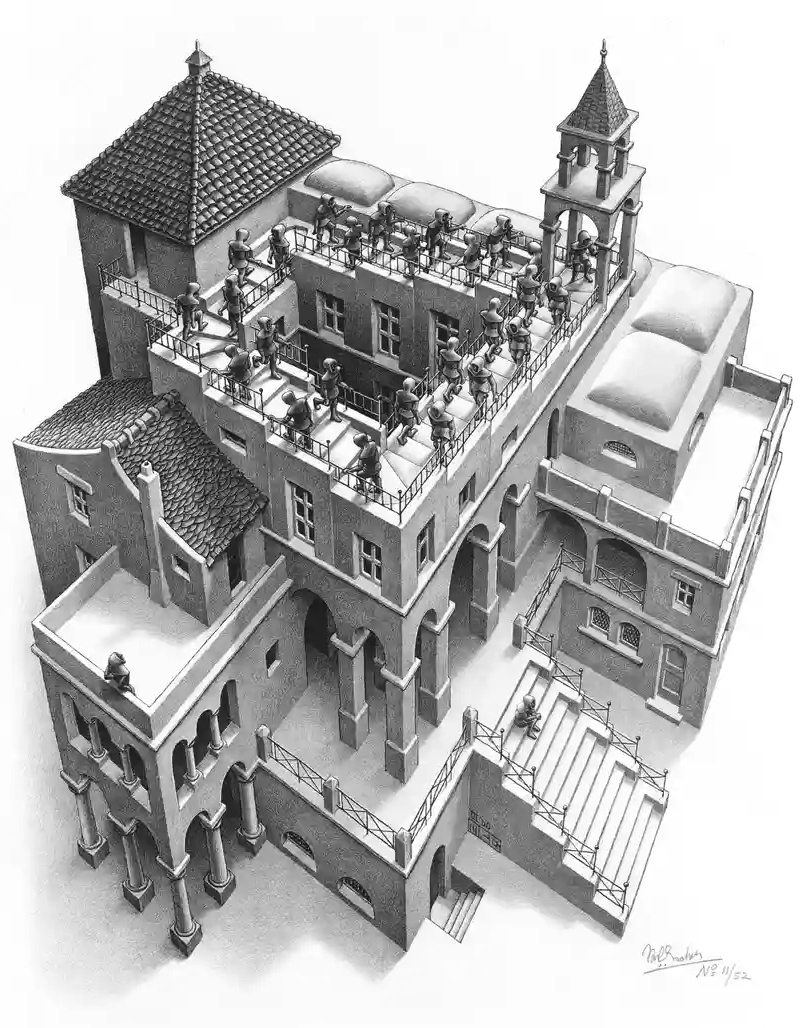
\includegraphics[width=1.05\columnwidth]{figures/penrose-stairs.png}
	\caption{
		\emph{``Ascending and Descending'' by M.\ C.\ Escher, 1960} --- perhaps the most famous illustration of an inexact $2$-form (the slope of the stairs) and its inconsistent `integral' (the impossible staircase).
	}
\end{marginfigure}
We can also translate the involutivity condition from tangent subbundles to ideals.
\begin{theorem}
	\label{thm:dual-involutive}
	If $𝒟 ⊆ \TTℳ$ is a tangent subbundle and $I ⊆ \forms[1](ℳ)$ is its associated ideal, then
	\begin{align}
		[𝒟, 𝒟] ⊆ 𝒟
		\quad ⟺ \quad
		\text{$𝒟$ is involutive}
		\quad ⟺ \quad
		\dd I ⊆ I
	.\end{align}
\end{theorem}
\begin{proof}
	The first equivalence is by definition, included for readability.
	For the second, note that the ideal $I$ is generated by $1$-forms $ω$ which vanish on $𝒟$.
	That is, $ω(𝒖) = 0$ for all $𝒖 ∈ \secs(𝒟)$, so if $𝒖, 𝒗 ∈ \secs(𝒟)$ then
	\begin{align}
		\label{eqn:xd-lb-identity}
		\dd ω(𝒖, 𝒗) &= 𝒖\qty(ω(𝒗)) - 𝒗\qty(ω(𝒖)) - ω([𝒖, 𝒗])
	\\	&= - ω([𝒖, 𝒗])
	,\end{align}
	since $ω(𝒖) = ω(𝒗) = 0$.
	If $𝒟$ is involutive then $[𝒖, 𝒗] ∈ \secs(𝒟)$ and $\dd ω(𝒖, 𝒗) = 0$.
	Thus, $\dd ω ∈ I$ if and only if $𝒟$ is involutive.
\end{proof}

Hence, by \cref{thm:Frobenius,thm:dual-involutive}, a tangent subbundle admits maximal integral surfaces if and only if its associated ideal $I$ is closed under exterior differentiation, $\dd I ⊆ I$.

Stokes’ \cref{thm:flat-stokes} states that a differential form $φ$ is integrable if it is exact (i.e., if $φ = \dd ϕ$).
On a contractible domain, this is equivalent to $φ$ being closed, by Poincaré's lemma.
In the same vein, \cref{thm:dual-involutive} states that an exterior differential system is integrable over a contractible domain if and only if its associated ideal is closed.




\subsection{Curvature as an obstruction to integrability}




We may employ Frobenius’ theorem to find the integrability condition for the connection on a vector bundle $\fibrebundle V 𝒱 ℳ$.
A linear Ehresmann connection $H$ is integrable if there exist maximal integral manifolds $f ∈ \secs(ℱ)$ which are everywhere horizontal, $\TT_p f = H_p$.
This means that $∇ f = 0$ everywhere, that parallel transport is path-independent, and that loop holonomy is always trivial.

Elaborating the condition $∇ f = 0$, we have
\begin{align}
	\label{eqn:covariantly-const}
	∇_𝒖 X = 𝒖(X) + Γ(𝒖)X = 0
	\qqtext{or}
	∂_μ X^a = -Γ_μ{}^a{}_b X^b
\end{align}
everywhere for all $𝒖 ∈ \TT ℳ$.
These equations describe the tangent subbundle $H$.
To express this, introduce coordinates $\set{x^μ}$ of $ℳ$ and linear coordinates $\set{x^a}$ of $V$ with respect to some basis.
A point $X ∈ 𝒱$ is a base point $π(X) ≡ (X^μ) ∈ ℳ$ together with a fibre value $(X^a) ∈ V$, having total coordinates
\begin{math}
	X = (X^μ, X^a)
.\end{math}
Similarly, a vector in $\TT_X 𝒱$ has components
\begin{math}
	δX = (δX^μ, δX^a)
.\end{math}

Such a vector $δX ∈ \TT_X 𝒱$ satisfies \cref{eqn:covariantly-const} if $δX^a/δX^μ = -Γ_μ{}^a{}_b X^b$, and hence the Ehresmann connection may be expressed as
\begin{align}
	\label{eqn:parallel-transport-tangent-subbundle}
	H_X = \spanof{(δX^μ, -Γ_μ{}^a{}_b X^b δX^μ) | (δX^μ) ∈ \TT_Xℳ}
\end{align}
for each $X ∈ 𝒱$.
Geometrically, this describes the change in vector components $δX^a$ induced by a nudge in the base point $δX^μ$ if $X$ is constrained to move along $H$.

To employ Frobenius’ theorem, we will find a dual representation of \cref{eqn:parallel-transport-tangent-subbundle} in terms of forms.
Any $X ∈ H$ is of the form
\begin{align}
	X = δX^μ(\∂_μ - Γ_μ{}^a{}_b X^b \∂_a)
.\end{align}
If $I$ is the ideal associated to $H$, then any $1$-form $\df ω ∈ I$ satisfies
\begin{align}
	\df ω(X) = δX^μ\qty(ω_μ - Γ_μ{}^a{}_b X^b ω_a) = 0
\end{align}
where $ω_A ≔ \df ω(\∂_A)$, implying $ω_μ =  Γ_μ{}^a{}_b X^b ω_a$ at $X$.
Written in the coordinate dual basis $\set{\df{\dd X}^μ, \df{\dd X}^a} ⊂ \TT^* 𝒱$,
\begin{align}
	\label{eqn:arbitrary-1-form-gen}
	\df ω = ω_a\qty(\df{\dd X}^a + Γ_μ{}^a{}_b X^b \df{\dd X}^μ)
\end{align}
where $ω_a$ are free scalar parameters.
Here, we adopt the notation `$\df{\phantom{ω}}$' to label differential forms for clarity.
Since \cref{eqn:arbitrary-1-form-gen} is a general $1$-form of the ideal $I$, we can see that $I$ is generated by the $1$-forms
\begin{align}
	\label{eqn:ideal-gens}
	\df Ω^a = \df{\dd X}^a + \df Γ^a{}_b X^b
,\end{align}
where we define the connection $1$-forms $\df Γ^a{}_b ≔ Γ_μ{}^a{}_b \, \df{\dd X}^μ$.

The dual formulation of Frobenius’ theorem (\cref{thm:dual-involutive}) states that the tangent subbundle $H$ is involuted if and only if the ideal $I$ is closed.
This means that $\dd \df Ω^a ∈ \dd I$ for every generator, which is equivalent to the condition $\dd\df Ω^a = \df α_a ∧ \df Ω^a$ for arbitrary `component $1$-forms' $\df α_a$.
By direct calculation,
\begin{align}
	\dd\df Ω^a &= \df{\dd^2 X^a} + \dd \df Γ^a{}_b X^b - \df Γ^a{}_b ∧ \df{\dd X^b}
\\	&= (\dd \df Γ^a{}_b + \df Γ^a{}_c ∧ \df Γ^c{}_b) X^b - \df Γ^a{}_b ∧ \df Ω^a
\end{align}
where we substitute \cref{eqn:ideal-gens} on the second line.
Therefore, $\dd\df Ω^a ∈ I$ if and only if the residual term, called the \textdef{connection $2$-form}
\begin{align}
	\df R^a{}_b ≔ \dd \df Γ^a{}_b + \df Γ^a{}_c ∧ \df Γ^c{}_b
,\end{align}
vanishes.
These $\df R^a{}_b$ measure the obstruction to integrability of the covariant derivative, and are identified as the primary object describing the connection's curvature.